% Generated by Sphinx.
\def\sphinxdocclass{report}
\documentclass[a4paper,10pt,english]{sphinxmanual}
\usepackage[utf8]{inputenc}
\DeclareUnicodeCharacter{00A0}{\nobreakspace}
\usepackage{cmap}
\usepackage[T1]{fontenc}
\usepackage{babel}
\usepackage{times}
\usepackage[Bjarne]{fncychap}
\usepackage{longtable}
\usepackage{sphinx}
\usepackage{multirow}

\addto\captionsenglish{\renewcommand{\figurename}{Fig. }}
\addto\captionsenglish{\renewcommand{\tablename}{Table }}
\floatname{literal-block}{Listing }



\title{Aqserver Documentation}
\date{October 20, 2016}
\release{1a}
\author{Michael Taxis}
\newcommand{\sphinxlogo}{}
\renewcommand{\releasename}{Release}
\makeindex

\makeatletter
\def\PYG@reset{\let\PYG@it=\relax \let\PYG@bf=\relax%
    \let\PYG@ul=\relax \let\PYG@tc=\relax%
    \let\PYG@bc=\relax \let\PYG@ff=\relax}
\def\PYG@tok#1{\csname PYG@tok@#1\endcsname}
\def\PYG@toks#1+{\ifx\relax#1\empty\else%
    \PYG@tok{#1}\expandafter\PYG@toks\fi}
\def\PYG@do#1{\PYG@bc{\PYG@tc{\PYG@ul{%
    \PYG@it{\PYG@bf{\PYG@ff{#1}}}}}}}
\def\PYG#1#2{\PYG@reset\PYG@toks#1+\relax+\PYG@do{#2}}

\expandafter\def\csname PYG@tok@gd\endcsname{\def\PYG@tc##1{\textcolor[rgb]{0.63,0.00,0.00}{##1}}}
\expandafter\def\csname PYG@tok@gu\endcsname{\let\PYG@bf=\textbf\def\PYG@tc##1{\textcolor[rgb]{0.50,0.00,0.50}{##1}}}
\expandafter\def\csname PYG@tok@gt\endcsname{\def\PYG@tc##1{\textcolor[rgb]{0.00,0.27,0.87}{##1}}}
\expandafter\def\csname PYG@tok@gs\endcsname{\let\PYG@bf=\textbf}
\expandafter\def\csname PYG@tok@gr\endcsname{\def\PYG@tc##1{\textcolor[rgb]{1.00,0.00,0.00}{##1}}}
\expandafter\def\csname PYG@tok@cm\endcsname{\let\PYG@it=\textit\def\PYG@tc##1{\textcolor[rgb]{0.25,0.50,0.56}{##1}}}
\expandafter\def\csname PYG@tok@vg\endcsname{\def\PYG@tc##1{\textcolor[rgb]{0.73,0.38,0.84}{##1}}}
\expandafter\def\csname PYG@tok@m\endcsname{\def\PYG@tc##1{\textcolor[rgb]{0.13,0.50,0.31}{##1}}}
\expandafter\def\csname PYG@tok@mh\endcsname{\def\PYG@tc##1{\textcolor[rgb]{0.13,0.50,0.31}{##1}}}
\expandafter\def\csname PYG@tok@cs\endcsname{\def\PYG@tc##1{\textcolor[rgb]{0.25,0.50,0.56}{##1}}\def\PYG@bc##1{\setlength{\fboxsep}{0pt}\colorbox[rgb]{1.00,0.94,0.94}{\strut ##1}}}
\expandafter\def\csname PYG@tok@ge\endcsname{\let\PYG@it=\textit}
\expandafter\def\csname PYG@tok@vc\endcsname{\def\PYG@tc##1{\textcolor[rgb]{0.73,0.38,0.84}{##1}}}
\expandafter\def\csname PYG@tok@il\endcsname{\def\PYG@tc##1{\textcolor[rgb]{0.13,0.50,0.31}{##1}}}
\expandafter\def\csname PYG@tok@go\endcsname{\def\PYG@tc##1{\textcolor[rgb]{0.20,0.20,0.20}{##1}}}
\expandafter\def\csname PYG@tok@cp\endcsname{\def\PYG@tc##1{\textcolor[rgb]{0.00,0.44,0.13}{##1}}}
\expandafter\def\csname PYG@tok@gi\endcsname{\def\PYG@tc##1{\textcolor[rgb]{0.00,0.63,0.00}{##1}}}
\expandafter\def\csname PYG@tok@gh\endcsname{\let\PYG@bf=\textbf\def\PYG@tc##1{\textcolor[rgb]{0.00,0.00,0.50}{##1}}}
\expandafter\def\csname PYG@tok@ni\endcsname{\let\PYG@bf=\textbf\def\PYG@tc##1{\textcolor[rgb]{0.84,0.33,0.22}{##1}}}
\expandafter\def\csname PYG@tok@nl\endcsname{\let\PYG@bf=\textbf\def\PYG@tc##1{\textcolor[rgb]{0.00,0.13,0.44}{##1}}}
\expandafter\def\csname PYG@tok@nn\endcsname{\let\PYG@bf=\textbf\def\PYG@tc##1{\textcolor[rgb]{0.05,0.52,0.71}{##1}}}
\expandafter\def\csname PYG@tok@no\endcsname{\def\PYG@tc##1{\textcolor[rgb]{0.38,0.68,0.84}{##1}}}
\expandafter\def\csname PYG@tok@na\endcsname{\def\PYG@tc##1{\textcolor[rgb]{0.25,0.44,0.63}{##1}}}
\expandafter\def\csname PYG@tok@nb\endcsname{\def\PYG@tc##1{\textcolor[rgb]{0.00,0.44,0.13}{##1}}}
\expandafter\def\csname PYG@tok@nc\endcsname{\let\PYG@bf=\textbf\def\PYG@tc##1{\textcolor[rgb]{0.05,0.52,0.71}{##1}}}
\expandafter\def\csname PYG@tok@nd\endcsname{\let\PYG@bf=\textbf\def\PYG@tc##1{\textcolor[rgb]{0.33,0.33,0.33}{##1}}}
\expandafter\def\csname PYG@tok@ne\endcsname{\def\PYG@tc##1{\textcolor[rgb]{0.00,0.44,0.13}{##1}}}
\expandafter\def\csname PYG@tok@nf\endcsname{\def\PYG@tc##1{\textcolor[rgb]{0.02,0.16,0.49}{##1}}}
\expandafter\def\csname PYG@tok@si\endcsname{\let\PYG@it=\textit\def\PYG@tc##1{\textcolor[rgb]{0.44,0.63,0.82}{##1}}}
\expandafter\def\csname PYG@tok@s2\endcsname{\def\PYG@tc##1{\textcolor[rgb]{0.25,0.44,0.63}{##1}}}
\expandafter\def\csname PYG@tok@vi\endcsname{\def\PYG@tc##1{\textcolor[rgb]{0.73,0.38,0.84}{##1}}}
\expandafter\def\csname PYG@tok@nt\endcsname{\let\PYG@bf=\textbf\def\PYG@tc##1{\textcolor[rgb]{0.02,0.16,0.45}{##1}}}
\expandafter\def\csname PYG@tok@nv\endcsname{\def\PYG@tc##1{\textcolor[rgb]{0.73,0.38,0.84}{##1}}}
\expandafter\def\csname PYG@tok@s1\endcsname{\def\PYG@tc##1{\textcolor[rgb]{0.25,0.44,0.63}{##1}}}
\expandafter\def\csname PYG@tok@gp\endcsname{\let\PYG@bf=\textbf\def\PYG@tc##1{\textcolor[rgb]{0.78,0.36,0.04}{##1}}}
\expandafter\def\csname PYG@tok@sh\endcsname{\def\PYG@tc##1{\textcolor[rgb]{0.25,0.44,0.63}{##1}}}
\expandafter\def\csname PYG@tok@ow\endcsname{\let\PYG@bf=\textbf\def\PYG@tc##1{\textcolor[rgb]{0.00,0.44,0.13}{##1}}}
\expandafter\def\csname PYG@tok@sx\endcsname{\def\PYG@tc##1{\textcolor[rgb]{0.78,0.36,0.04}{##1}}}
\expandafter\def\csname PYG@tok@bp\endcsname{\def\PYG@tc##1{\textcolor[rgb]{0.00,0.44,0.13}{##1}}}
\expandafter\def\csname PYG@tok@c1\endcsname{\let\PYG@it=\textit\def\PYG@tc##1{\textcolor[rgb]{0.25,0.50,0.56}{##1}}}
\expandafter\def\csname PYG@tok@kc\endcsname{\let\PYG@bf=\textbf\def\PYG@tc##1{\textcolor[rgb]{0.00,0.44,0.13}{##1}}}
\expandafter\def\csname PYG@tok@c\endcsname{\let\PYG@it=\textit\def\PYG@tc##1{\textcolor[rgb]{0.25,0.50,0.56}{##1}}}
\expandafter\def\csname PYG@tok@mf\endcsname{\def\PYG@tc##1{\textcolor[rgb]{0.13,0.50,0.31}{##1}}}
\expandafter\def\csname PYG@tok@err\endcsname{\def\PYG@bc##1{\setlength{\fboxsep}{0pt}\fcolorbox[rgb]{1.00,0.00,0.00}{1,1,1}{\strut ##1}}}
\expandafter\def\csname PYG@tok@mb\endcsname{\def\PYG@tc##1{\textcolor[rgb]{0.13,0.50,0.31}{##1}}}
\expandafter\def\csname PYG@tok@ss\endcsname{\def\PYG@tc##1{\textcolor[rgb]{0.32,0.47,0.09}{##1}}}
\expandafter\def\csname PYG@tok@sr\endcsname{\def\PYG@tc##1{\textcolor[rgb]{0.14,0.33,0.53}{##1}}}
\expandafter\def\csname PYG@tok@mo\endcsname{\def\PYG@tc##1{\textcolor[rgb]{0.13,0.50,0.31}{##1}}}
\expandafter\def\csname PYG@tok@kd\endcsname{\let\PYG@bf=\textbf\def\PYG@tc##1{\textcolor[rgb]{0.00,0.44,0.13}{##1}}}
\expandafter\def\csname PYG@tok@mi\endcsname{\def\PYG@tc##1{\textcolor[rgb]{0.13,0.50,0.31}{##1}}}
\expandafter\def\csname PYG@tok@kn\endcsname{\let\PYG@bf=\textbf\def\PYG@tc##1{\textcolor[rgb]{0.00,0.44,0.13}{##1}}}
\expandafter\def\csname PYG@tok@o\endcsname{\def\PYG@tc##1{\textcolor[rgb]{0.40,0.40,0.40}{##1}}}
\expandafter\def\csname PYG@tok@kr\endcsname{\let\PYG@bf=\textbf\def\PYG@tc##1{\textcolor[rgb]{0.00,0.44,0.13}{##1}}}
\expandafter\def\csname PYG@tok@s\endcsname{\def\PYG@tc##1{\textcolor[rgb]{0.25,0.44,0.63}{##1}}}
\expandafter\def\csname PYG@tok@kp\endcsname{\def\PYG@tc##1{\textcolor[rgb]{0.00,0.44,0.13}{##1}}}
\expandafter\def\csname PYG@tok@w\endcsname{\def\PYG@tc##1{\textcolor[rgb]{0.73,0.73,0.73}{##1}}}
\expandafter\def\csname PYG@tok@kt\endcsname{\def\PYG@tc##1{\textcolor[rgb]{0.56,0.13,0.00}{##1}}}
\expandafter\def\csname PYG@tok@sc\endcsname{\def\PYG@tc##1{\textcolor[rgb]{0.25,0.44,0.63}{##1}}}
\expandafter\def\csname PYG@tok@sb\endcsname{\def\PYG@tc##1{\textcolor[rgb]{0.25,0.44,0.63}{##1}}}
\expandafter\def\csname PYG@tok@k\endcsname{\let\PYG@bf=\textbf\def\PYG@tc##1{\textcolor[rgb]{0.00,0.44,0.13}{##1}}}
\expandafter\def\csname PYG@tok@se\endcsname{\let\PYG@bf=\textbf\def\PYG@tc##1{\textcolor[rgb]{0.25,0.44,0.63}{##1}}}
\expandafter\def\csname PYG@tok@sd\endcsname{\let\PYG@it=\textit\def\PYG@tc##1{\textcolor[rgb]{0.25,0.44,0.63}{##1}}}

\def\PYGZbs{\char`\\}
\def\PYGZus{\char`\_}
\def\PYGZob{\char`\{}
\def\PYGZcb{\char`\}}
\def\PYGZca{\char`\^}
\def\PYGZam{\char`\&}
\def\PYGZlt{\char`\<}
\def\PYGZgt{\char`\>}
\def\PYGZsh{\char`\#}
\def\PYGZpc{\char`\%}
\def\PYGZdl{\char`\$}
\def\PYGZhy{\char`\-}
\def\PYGZsq{\char`\'}
\def\PYGZdq{\char`\"}
\def\PYGZti{\char`\~}
% for compatibility with earlier versions
\def\PYGZat{@}
\def\PYGZlb{[}
\def\PYGZrb{]}
\makeatother

\renewcommand\PYGZsq{\textquotesingle}

\begin{document}

\maketitle
\tableofcontents
\phantomsection\label{index::doc}


The program is an acquisition tool for Siemens Simatic S7 PLCs.
It was written using the python-snap7 module from \href{https://pypi.python.org/pypi/python-snap7/}{https://pypi.python.org/pypi/python-snap7/} and the snap7 library from \href{http://snap7.sourceforge.net}{http://snap7.sourceforge.net} .
File handling is based on example source code for the book ``Real-World Instrumentation with Python''.
\begin{quote}\begin{description}
\item[{Homepage}] \leavevmode
\href{http://www.taxis-instruments.de}{http://www.taxis-instruments.de}

\item[{Contact}] \leavevmode
\textless{}aqserver at taxis-instruments dot de\textgreater{}

\item[{Author}] \leavevmode
Michael Taxis \textless{}michael at taxis-instruments dot de\textgreater{}

\end{description}\end{quote}

Copyright of this document:
\begin{quote}\begin{description}
\item[{Copyright}] \leavevmode
\href{http://creativecommons.org/licenses/by-sa/3.0/}{CC BY-SA 3.0}

\end{description}\end{quote}

Copyright of the program:
\begin{quote}\begin{description}
\item[{Copyright}] \leavevmode
\href{https://www.gnu.org/licenses/lgpl-3.0-standalone.html}{LESSER GNU GENERAL PUBLIC LICENSE 3.0}

\end{description}\end{quote}

Please note that soft- and hardware designations and brand names of their respective companies  used in this document are  generally subject to trademark protection or patent protection.


\chapter{About}
\label{about:about}\label{about:aqserver-siemens-s7-data-acquisition-server}\label{about::doc}
With this program you can record values from a Simatic S7 PLC to a CSV File. Depending on the number of values to record the scan time is changing, thus increasing with the number of values. It is possible to set trigger conditions, that will start a new file. The old file will be compressed and stored in a selectable directory tree.
Using a pre- and post trigger time, you can set an overlap of old and new file. If you are not able to set a working trigger, the trigger can also be activated manually.

A config file must exist (default file is aqserver.cfg) that defines communication and other parameters and of course the S7 variables to scan. Open the config file in your preferred editor and read the comments on how to
configure.

Values will be stored to a csv-file in subdirectory data. Filename can be specified in configfile. Once a configurable trigger is raised, a new datafile begins.

After trigger or when program is stopped, the data file will be compressed and stored to a path, that can also be specified in the config file.

When running several instances of the program, using different config files, values can be recorded from different PLCs at the same time.

Please note that this program is in an early stage of development. If you run into problems when using it, see the ``Problems'' section of this manual. Aqserver will not create a problem with your PLC program though.

Using Kst2 from \href{https://kst-plot.kde.org}{https://kst-plot.kde.org} the datafile can be read and plotted online during the recording. Also decompressed archives can be plotted to your liking.

An alternative would be LiveGraph from \href{http://www.live-graph.org}{http://www.live-graph.org} , but then the data files must be modified, because LiveGraph is expecting csv-files in a certain format (actually this is not provided by Aqserver at the moment).


\chapter{Installation}
\label{installation:installation}\label{installation::doc}
Program can be obtained from \href{http://www.taxis-instruments.de}{http://www.taxis-instruments.de} .

The program was written using Python 2.7.10 under Windows 7 - 32 bit.


\section{Install from source}
\label{installation:install-from-source}
If you would like to run from the python source you must have a working Python 2.7 installation. For a full working Python environment I can recommend the Python (x,y) distribution from \href{https://python-xy.github.io/}{https://python-xy.github.io/} or Winpython from \href{https://winpython.github.io/}{https://winpython.github.io/} for a Windows environment (just make sure you are using the latest Python 2 package). On Linux and MacOS environments Python should already be installed as part of the OS.

Program is using (at least parts of) the following Python libraries (not in any particular order..):
\begin{itemize}
\item {} 
time

\item {} 
sys

\item {} 
os

\item {} 
shutil

\item {} 
ctypes

\item {} 
struct

\item {} 
logging

\item {} 
collections

\item {} 
win32com

\item {} 
python-snap7

\item {} 
socket

\item {} 
datetime

\item {} 
gzip

\item {} 
bz2

\item {} 
binascii

\item {} 
ConfigParser

\item {} 
distutils

\end{itemize}

This libraries can be installed with pip.

Python-snap7 is a python wrapper for snap7 from \href{http://snap7.sourceforge.net/}{http://snap7.sourceforge.net/}. So make sure you have a working copy of this also on your machine.


\section{Install with Windows Installer}
\label{installation:install-with-windows-installer}
To install the program you can use the provided installer. Run setup.exe as Administrator and follow instructions of the installer. A link to the program will be installed into the startmenu.
The program will be installed to the directory ``C:\textbackslash{}Program Files (x86)\textbackslash{}Aqserver\textbackslash{}''. Additionally the folder ``Aqserver'' plus sub folders ``help'', ``log'' and ``data'' will be created in the My Documents folder of the current user.
In the ``Aqserver'' directory you will find the following files:
\begin{itemize}
\item {} 
test.bat: a Windows / DOS batch file that will start Aqserver with the test configuration. You can copy and edit this file to personalize it for different configuration. I am also using this to start Aqserver from Windows Explorer or to run multiple instances (one batch file per instance)

\item {} 
test.cfg: an example config file that you can edit to match your requirements (good idea is to make a copy first..)

\end{itemize}

To uninstall run the uninstaller from the startmenu or uninstall from windows control panel.


\section{Manual installation}
\label{installation:manual-installation}
To install the program in a Windows Environment without a working Python installation use a folder of your liking and copy the files aqserver.exe, aqserver.cfg, aqserver.chm and aqserver.pdf to this folder. Copy snap7.dll to your Windows\textbackslash{}system32 directory. That's all. No install or setup procedure.
To remove the program just delete these files from your system. Nothing will remain.


\chapter{Configuration file for data acquisition server}
\label{configuration:configuration-file-for-data-acquisition-server}\label{configuration::doc}
In order to run Aqserver you need a configuration file where all required parameters for a acquisition from a S7PLC are stored.  When Aqserver is starting, this configuration is scanned, the parameters a re checked for correctness, then the acquisition starts.


\section{Prerequisites}
\label{configuration:prerequisites}
Multiline settings must be indented with TAB, see ``remarks''

In config file comments start with a ``\#'':
``\#'' at 1st column of line will be a comment, you can also use it to disable settings. Note
that always one valid setting must be available

Use '';'' for inline comments

Multiline comments must be indented with TAB, see ``remarks'':
If you want to have some text in more than one line, following lines must
be indented with TAB, see remarks in aqdata settings


\section{Settings in config file}
\label{configuration:settings-in-config-file}

\subsection{Aqdata settings}
\label{configuration:aqdata-settings}
For information purposes, we can set some texts, that will be included in the data file header.
You can add a text by placing the name starting in the first column followed by a ``='' and the text you wish to be implemented.

\begin{notice}{note}{Note:}
Also all config values are included in the datafile. When you open an de-archived datafile, you can copy these to make the same config file, if you have lost the original one.
\end{notice}

\begin{Verbatim}[commandchars=\\\{\}]
\PYGZsh{}\PYGZsh{}\PYGZsh{}\PYGZsh{}\PYGZsh{}\PYGZsh{}\PYGZsh{}\PYGZsh{}\PYGZsh{}\PYGZsh{}\PYGZsh{}\PYGZsh{}\PYGZsh{}\PYGZsh{}\PYGZsh{}\PYGZsh{}\PYGZsh{}\PYGZsh{}\PYGZsh{}\PYGZsh{}\PYGZsh{}\PYGZsh{}\PYGZsh{}\PYGZsh{}\PYGZsh{}\PYGZsh{}\PYGZsh{}\PYGZsh{}\PYGZsh{}\PYGZsh{}\PYGZsh{}\PYGZsh{}\PYGZsh{}\PYGZsh{}\PYGZsh{}\PYGZsh{}\PYGZsh{}\PYGZsh{}\PYGZsh{}\PYGZsh{}\PYGZsh{}\PYGZsh{}\PYGZsh{}\PYGZsh{}\PYGZsh{}\PYGZsh{}\PYGZsh{}\PYGZsh{}\PYGZsh{}\PYGZsh{}\PYGZsh{}\PYGZsh{}\PYGZsh{}\PYGZsh{}\PYGZsh{}\PYGZsh{}\PYGZsh{}\PYGZsh{}\PYGZsh{}\PYGZsh{}\PYGZsh{}\PYGZsh{}\PYGZsh{}\PYGZsh{}\PYGZsh{}\PYGZsh{}\PYGZsh{}\PYGZsh{}\PYGZsh{}\PYGZsh{}\PYGZsh{}\PYGZsh{}
\PYGZsh{} aqdata settings
\PYGZsh{}\PYGZsh{}\PYGZsh{}\PYGZsh{}\PYGZsh{}\PYGZsh{}\PYGZsh{}\PYGZsh{}\PYGZsh{}\PYGZsh{}\PYGZsh{}\PYGZsh{}\PYGZsh{}\PYGZsh{}\PYGZsh{}\PYGZsh{}\PYGZsh{}\PYGZsh{}\PYGZsh{}\PYGZsh{}\PYGZsh{}\PYGZsh{}\PYGZsh{}\PYGZsh{}\PYGZsh{}\PYGZsh{}\PYGZsh{}\PYGZsh{}\PYGZsh{}\PYGZsh{}\PYGZsh{}\PYGZsh{}\PYGZsh{}\PYGZsh{}\PYGZsh{}\PYGZsh{}\PYGZsh{}\PYGZsh{}\PYGZsh{}\PYGZsh{}\PYGZsh{}\PYGZsh{}\PYGZsh{}\PYGZsh{}\PYGZsh{}\PYGZsh{}\PYGZsh{}\PYGZsh{}\PYGZsh{}\PYGZsh{}\PYGZsh{}\PYGZsh{}\PYGZsh{}\PYGZsh{}\PYGZsh{}\PYGZsh{}\PYGZsh{}\PYGZsh{}\PYGZsh{}\PYGZsh{}\PYGZsh{}\PYGZsh{}\PYGZsh{}\PYGZsh{}\PYGZsh{}\PYGZsh{}\PYGZsh{}\PYGZsh{}\PYGZsh{}\PYGZsh{}\PYGZsh{}\PYGZsh{}
[aqdata]
place = somewhere

creator = Michael Taxis

machine = MyMachine

order = 123456

yourText = type whatever you desire

remarks = ; use tab for multiline values
    trials with double spreader, to get rid of married rolls
    trials for SF production
\end{Verbatim}


\subsection{Communication settings}
\label{configuration:communication-settings}
For communication with S7 we need following parameters:
\begin{itemize}
\item {} 
IP address: IP address of the PLC you try to reach. Try a PING before you start!

\item {} 
rack number: normally is 0

\item {} 
slot number: normally is number left of CPU in HW configuration, in example in picture below it is 3.

\item {} 
maximum connection attempts: Program tries to connect to PLC. If it fails after this number of trials/attempts the program stops. Then check your configuration and connection. If the value is set to 0 the program will try forever. This can be useful if you have the program running without supervision. If not sucessful you can still stop it with CTRL-C. When communication is interrupted/disconnected during a recording session, it will try to reconnect. There will be no recording of values when disconnected.

\end{itemize}

{\hfill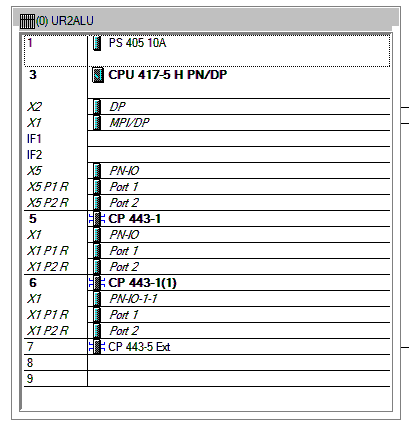
\includegraphics{hwconfig.png}\hfill}

\begin{Verbatim}[commandchars=\\\{\}]
\PYGZsh{}\PYGZsh{}\PYGZsh{}\PYGZsh{}\PYGZsh{}\PYGZsh{}\PYGZsh{}\PYGZsh{}\PYGZsh{}\PYGZsh{}\PYGZsh{}\PYGZsh{}\PYGZsh{}\PYGZsh{}\PYGZsh{}\PYGZsh{}\PYGZsh{}\PYGZsh{}\PYGZsh{}\PYGZsh{}\PYGZsh{}\PYGZsh{}\PYGZsh{}\PYGZsh{}\PYGZsh{}\PYGZsh{}\PYGZsh{}\PYGZsh{}\PYGZsh{}\PYGZsh{}\PYGZsh{}\PYGZsh{}\PYGZsh{}\PYGZsh{}\PYGZsh{}\PYGZsh{}\PYGZsh{}\PYGZsh{}\PYGZsh{}\PYGZsh{}\PYGZsh{}\PYGZsh{}\PYGZsh{}\PYGZsh{}\PYGZsh{}\PYGZsh{}\PYGZsh{}\PYGZsh{}\PYGZsh{}\PYGZsh{}\PYGZsh{}\PYGZsh{}\PYGZsh{}\PYGZsh{}\PYGZsh{}\PYGZsh{}\PYGZsh{}\PYGZsh{}\PYGZsh{}\PYGZsh{}\PYGZsh{}\PYGZsh{}\PYGZsh{}\PYGZsh{}\PYGZsh{}\PYGZsh{}\PYGZsh{}\PYGZsh{}\PYGZsh{}\PYGZsh{}\PYGZsh{}\PYGZsh{}
\PYGZsh{} communication settings
\PYGZsh{}\PYGZsh{}\PYGZsh{}\PYGZsh{}\PYGZsh{}\PYGZsh{}\PYGZsh{}\PYGZsh{}\PYGZsh{}\PYGZsh{}\PYGZsh{}\PYGZsh{}\PYGZsh{}\PYGZsh{}\PYGZsh{}\PYGZsh{}\PYGZsh{}\PYGZsh{}\PYGZsh{}\PYGZsh{}\PYGZsh{}\PYGZsh{}\PYGZsh{}\PYGZsh{}\PYGZsh{}\PYGZsh{}\PYGZsh{}\PYGZsh{}\PYGZsh{}\PYGZsh{}\PYGZsh{}\PYGZsh{}\PYGZsh{}\PYGZsh{}\PYGZsh{}\PYGZsh{}\PYGZsh{}\PYGZsh{}\PYGZsh{}\PYGZsh{}\PYGZsh{}\PYGZsh{}\PYGZsh{}\PYGZsh{}\PYGZsh{}\PYGZsh{}\PYGZsh{}\PYGZsh{}\PYGZsh{}\PYGZsh{}\PYGZsh{}\PYGZsh{}\PYGZsh{}\PYGZsh{}\PYGZsh{}\PYGZsh{}\PYGZsh{}\PYGZsh{}\PYGZsh{}\PYGZsh{}\PYGZsh{}\PYGZsh{}\PYGZsh{}\PYGZsh{}\PYGZsh{}\PYGZsh{}\PYGZsh{}\PYGZsh{}\PYGZsh{}\PYGZsh{}\PYGZsh{}\PYGZsh{}
[communication]

\PYGZsh{} setting up communication parameters to S7\PYGZhy{}PLC

\PYGZsh{} IP address
\PYGZsh{} you can leave several settings , just comment with a leading \PYGZdq{}\PYGZsh{}\PYGZdq{}
\PYGZsh{}IP = 192.168.1.107
IP = 172.16.13.174

\PYGZsh{} rack number, see HW Config
RACK = 0

\PYGZsh{} slot number of CPU, see HW Config
SLOT = 3

\PYGZsh{} maximum attempts for connection, 0 is trying forever
maxattempts = 10
\end{Verbatim}

\begin{notice}{note}{Note:}
You can also try Aqserver with PLCSIM and NetToPlcsim from \href{http://nettoplcsim.sourceforge.net/}{http://nettoplcsim.sourceforge.net/} on the same machine.
\end{notice}


\subsection{Miscellaneous settings}
\label{configuration:miscellaneous-settings}
We need some general settings for aqserver, as follows:
\begin{itemize}
\item {} 
delimiter: is the character that separates the recorded values in the data file, normally we use '';''. Be careful not to use the decimal separator that is used on your system (so don't use `.' or `,')!

\item {} 
datafileprefix: here we can define a name, that is used to identify the data file. It is a prefix, because file name also includes a timestamp e.g.: MyProject20150804\_173035.csv.gz

\item {} 
datafile is the filename, without extension, where actual data are recorded. This is a csv-file. If you intend to run multiple instances of the program, in order to reach different PLCs, make sure that this name is different in all config files!

\item {} 
autostart: defines whether recording is starting with program start, or is waiting for a start signal

\item {} 
datapath: here we define were the compressed data files will be stored.

\item {} 
usedir: defines, whether we use a directory structure as \textbackslash{}yyyy\textbackslash{}MM\textbackslash{}dd\textbackslash{} when storing the archived files.

\item {} 
scantime: scantime in milliseconds{[}ms{]}, minimum is limited to 20 ms in program. This time is only an approximation, because it also depends on number of variables to scan, but use it to reduce filesize. The more scans the bigger the file. If you set scantime to 0, the program will read the data as fast as possible (Attention: big data file!). Depending on the number of values scantime of \textasciitilde{}10 ms can be reached.

\item {} 
maxrecords: This number defines the maximum number of records stored to one file. This limit the size of a datafile. Depending on the number of values per record you should check what number is applicable for you.

\end{itemize}

\begin{Verbatim}[commandchars=\\\{\}]
\PYGZsh{}\PYGZsh{}\PYGZsh{}\PYGZsh{}\PYGZsh{}\PYGZsh{}\PYGZsh{}\PYGZsh{}\PYGZsh{}\PYGZsh{}\PYGZsh{}\PYGZsh{}\PYGZsh{}\PYGZsh{}\PYGZsh{}\PYGZsh{}\PYGZsh{}\PYGZsh{}\PYGZsh{}\PYGZsh{}\PYGZsh{}\PYGZsh{}\PYGZsh{}\PYGZsh{}\PYGZsh{}\PYGZsh{}\PYGZsh{}\PYGZsh{}\PYGZsh{}\PYGZsh{}\PYGZsh{}\PYGZsh{}\PYGZsh{}\PYGZsh{}\PYGZsh{}\PYGZsh{}\PYGZsh{}\PYGZsh{}\PYGZsh{}\PYGZsh{}\PYGZsh{}\PYGZsh{}\PYGZsh{}\PYGZsh{}\PYGZsh{}\PYGZsh{}\PYGZsh{}\PYGZsh{}\PYGZsh{}\PYGZsh{}\PYGZsh{}\PYGZsh{}\PYGZsh{}\PYGZsh{}\PYGZsh{}\PYGZsh{}\PYGZsh{}\PYGZsh{}\PYGZsh{}\PYGZsh{}\PYGZsh{}\PYGZsh{}\PYGZsh{}\PYGZsh{}\PYGZsh{}\PYGZsh{}\PYGZsh{}\PYGZsh{}\PYGZsh{}\PYGZsh{}\PYGZsh{}\PYGZsh{}
\PYGZsh{} miscellaneous settings
\PYGZsh{}\PYGZsh{}\PYGZsh{}\PYGZsh{}\PYGZsh{}\PYGZsh{}\PYGZsh{}\PYGZsh{}\PYGZsh{}\PYGZsh{}\PYGZsh{}\PYGZsh{}\PYGZsh{}\PYGZsh{}\PYGZsh{}\PYGZsh{}\PYGZsh{}\PYGZsh{}\PYGZsh{}\PYGZsh{}\PYGZsh{}\PYGZsh{}\PYGZsh{}\PYGZsh{}\PYGZsh{}\PYGZsh{}\PYGZsh{}\PYGZsh{}\PYGZsh{}\PYGZsh{}\PYGZsh{}\PYGZsh{}\PYGZsh{}\PYGZsh{}\PYGZsh{}\PYGZsh{}\PYGZsh{}\PYGZsh{}\PYGZsh{}\PYGZsh{}\PYGZsh{}\PYGZsh{}\PYGZsh{}\PYGZsh{}\PYGZsh{}\PYGZsh{}\PYGZsh{}\PYGZsh{}\PYGZsh{}\PYGZsh{}\PYGZsh{}\PYGZsh{}\PYGZsh{}\PYGZsh{}\PYGZsh{}\PYGZsh{}\PYGZsh{}\PYGZsh{}\PYGZsh{}\PYGZsh{}\PYGZsh{}\PYGZsh{}\PYGZsh{}\PYGZsh{}\PYGZsh{}\PYGZsh{}\PYGZsh{}\PYGZsh{}\PYGZsh{}\PYGZsh{}\PYGZsh{}\PYGZsh{}
[misc]

\PYGZsh{} miscellaneous values for setting up the acquisition server
\PYGZsh{} value delimiter in storage file
delimiter = ;

\PYGZsh{} prefix of data file name, e.g. a customer/project name or whatever
datafileprefix = MyProject

\PYGZsh{} data file name for actual data recording, without extension!
\PYGZsh{} e.g. if you use \PYGZdq{}filename\PYGZdq{}, actual name will be \PYGZdq{}filename.csv\PYGZdq{}
datafile = recording

\PYGZsh{} autostart: when program is started decide whether acquisition is started(1)
\PYGZsh{} immediately or wait for start signal (0)
autostart = 0

\PYGZsh{} path for data files, use \PYGZdq{}\PYGZbs{}\PYGZdq{} for directory separation, with \PYGZdq{}\PYGZbs{}\PYGZdq{} at the end !
\PYGZsh{} e.g. datapath = D:\PYGZbs{}mydata\PYGZbs{}
datapath = F:\PYGZbs{}aqdata\PYGZbs{}MyProject\PYGZbs{}

\PYGZsh{} if 1 use directory structure datapath\PYGZbs{}yyyyy\PYGZbs{}MM\PYGZbs{}dd otherwise use only datapath
usedir = 1

\PYGZsh{} scantime in milliseconds [ms]
\PYGZsh{} if you just put 0 program will scan as fast as possible
\PYGZsh{} this will produce rather large data files!
\PYGZsh{} depending on number of values this value is just a hint ;\PYGZhy{})
scantime = 100

\PYGZsh{} maximum number of records
\PYGZsh{} to avoid too big data files, a new one will be starfted after this number
\PYGZsh{} of recordings
maxrecords = 50000
\end{Verbatim}


\subsection{Trigger settings}
\label{configuration:trigger-settings}
Trigger settings are used to start a new datafile, when a trigger event occurs. A trigger can also be raised manually by pressing key `t' on your keyboard!
This trigger event is defined by the following three trigger settings:
\begin{itemize}
\item {} 
trgsignal: This is the ``name'' of the signal from the value section, that will trigger the event. Copy the name from the value section.

\item {} 
trgcondition: This the condition for a comparison of the triggersignal with the trigger value. E.g. when the condition is ``=='' then the trigger will be raised, when value of trigger signal and trigger value match

\item {} 
trgvalue: This is a constant, trgsignal is compared with it, to decide about the trigger event.

\end{itemize}

Further 2 values are used to overlap old and new file:
\begin{itemize}
\item {} 
pretrg: time that will be recorded to new file BEFORE the trigger in {[}s{]}. This is based on setting scantime.

\item {} 
posttrg: time that will be recorded to old file AFTER the trigger in {[}s{]}. This is based on setting scantime.

\end{itemize}

\begin{Verbatim}[commandchars=\\\{\}]
\PYGZsh{}\PYGZsh{}\PYGZsh{}\PYGZsh{}\PYGZsh{}\PYGZsh{}\PYGZsh{}\PYGZsh{}\PYGZsh{}\PYGZsh{}\PYGZsh{}\PYGZsh{}\PYGZsh{}\PYGZsh{}\PYGZsh{}\PYGZsh{}\PYGZsh{}\PYGZsh{}\PYGZsh{}\PYGZsh{}\PYGZsh{}\PYGZsh{}\PYGZsh{}\PYGZsh{}\PYGZsh{}\PYGZsh{}\PYGZsh{}\PYGZsh{}\PYGZsh{}\PYGZsh{}\PYGZsh{}\PYGZsh{}\PYGZsh{}\PYGZsh{}\PYGZsh{}\PYGZsh{}\PYGZsh{}\PYGZsh{}\PYGZsh{}\PYGZsh{}\PYGZsh{}\PYGZsh{}\PYGZsh{}\PYGZsh{}\PYGZsh{}\PYGZsh{}\PYGZsh{}\PYGZsh{}\PYGZsh{}\PYGZsh{}\PYGZsh{}\PYGZsh{}\PYGZsh{}\PYGZsh{}\PYGZsh{}\PYGZsh{}\PYGZsh{}\PYGZsh{}\PYGZsh{}\PYGZsh{}\PYGZsh{}\PYGZsh{}\PYGZsh{}\PYGZsh{}\PYGZsh{}\PYGZsh{}\PYGZsh{}\PYGZsh{}\PYGZsh{}\PYGZsh{}\PYGZsh{}\PYGZsh{}
\PYGZsh{} trigger settings
\PYGZsh{}\PYGZsh{}\PYGZsh{}\PYGZsh{}\PYGZsh{}\PYGZsh{}\PYGZsh{}\PYGZsh{}\PYGZsh{}\PYGZsh{}\PYGZsh{}\PYGZsh{}\PYGZsh{}\PYGZsh{}\PYGZsh{}\PYGZsh{}\PYGZsh{}\PYGZsh{}\PYGZsh{}\PYGZsh{}\PYGZsh{}\PYGZsh{}\PYGZsh{}\PYGZsh{}\PYGZsh{}\PYGZsh{}\PYGZsh{}\PYGZsh{}\PYGZsh{}\PYGZsh{}\PYGZsh{}\PYGZsh{}\PYGZsh{}\PYGZsh{}\PYGZsh{}\PYGZsh{}\PYGZsh{}\PYGZsh{}\PYGZsh{}\PYGZsh{}\PYGZsh{}\PYGZsh{}\PYGZsh{}\PYGZsh{}\PYGZsh{}\PYGZsh{}\PYGZsh{}\PYGZsh{}\PYGZsh{}\PYGZsh{}\PYGZsh{}\PYGZsh{}\PYGZsh{}\PYGZsh{}\PYGZsh{}\PYGZsh{}\PYGZsh{}\PYGZsh{}\PYGZsh{}\PYGZsh{}\PYGZsh{}\PYGZsh{}\PYGZsh{}\PYGZsh{}\PYGZsh{}\PYGZsh{}\PYGZsh{}\PYGZsh{}\PYGZsh{}\PYGZsh{}\PYGZsh{}\PYGZsh{}
\PYGZsh{} when trigger condition is matched, then we close the old file after
\PYGZsh{} post\PYGZhy{}trigger time and start the new file and copy pre\PYGZhy{}trigger time
\PYGZsh{} and post\PYGZhy{}trigger recordings to new file
\PYGZsh{}    \PYGZsh{} condition is, with example:
\PYGZsh{} trgsignal trgcondition trgvalue
\PYGZsh{} rewind diameter [mm] = 0
\PYGZsh{}
[trigger]

\PYGZsh{} trigger signal, copy the name of the signal in [values] section,
\PYGZsh{} that you want to use as trigger signal
trgsignal = rewind diameter [mm]

\PYGZsh{} trigger condition, use \PYGZgt{},\PYGZgt{}=,==, \PYGZlt{}=,\PYGZlt{},!= as condition
\PYGZsh{} when conditon is matched, then we close the old file and start a new one
\PYGZsh{} trgcondition = \PYGZgt{}
\PYGZsh{} trgcondition = \PYGZgt{}=
\PYGZsh{} trgcondition = ==
trgcondition = \PYGZlt{}=
\PYGZsh{} trgcondition = \PYGZlt{}
\PYGZsh{} trgcondition = !=

\PYGZsh{} trigger value, with this value we compare the trigger signal
trgvalue = 0

\PYGZsh{} pre\PYGZhy{}trigger time in seconds [s]
\PYGZsh{} will still add pre\PYGZhy{}trigger/scantime lines to old file after trigger event
\PYGZsh{} e.g. pre\PYGZhy{}trigger is 60 seconds and scantime is 100 ms, then 600 lines
\PYGZsh{} will be recorded after trigger event
pretrg = 30

\PYGZsh{}post\PYGZhy{}trigger time in seconds [s]
\PYGZsh{} will copy last post\PYGZhy{}trigger/scantime lines from old to new file
\PYGZsh{} e.g. post\PYGZhy{}trigger is 60 seconds and scantime is 100 ms, then 600 lines will
\PYGZsh{} be copied after trigger event
posttrg = 30
\end{Verbatim}


\subsection{Debug settings}
\label{configuration:debug-settings}
The debug settings define whether and how we do some logging to debug the program.

For debugging we have to define a debug level, that defines what will be logged.

With level ``0'' we switch off logging completely, with level ``1'' everything will be logged
Note that  when you restart the program the log directory will be purged,leaving only the latest log-file

Parameter logfile defines the name of the logfile, without extension.
Extension will always be ''.log''

If parameter logts is 1 everytime we start the program a new log file will be created. If logts is 0 then we will always append to the default log file.

\begin{Verbatim}[commandchars=\\\{\}]
\PYG{c}{\PYGZsh{}\PYGZsh{}\PYGZsh{}\PYGZsh{}\PYGZsh{}\PYGZsh{}\PYGZsh{}\PYGZsh{}\PYGZsh{}\PYGZsh{}\PYGZsh{}\PYGZsh{}\PYGZsh{}\PYGZsh{}\PYGZsh{}\PYGZsh{}\PYGZsh{}\PYGZsh{}\PYGZsh{}\PYGZsh{}\PYGZsh{}\PYGZsh{}\PYGZsh{}\PYGZsh{}\PYGZsh{}\PYGZsh{}\PYGZsh{}\PYGZsh{}\PYGZsh{}\PYGZsh{}\PYGZsh{}\PYGZsh{}\PYGZsh{}\PYGZsh{}\PYGZsh{}\PYGZsh{}\PYGZsh{}\PYGZsh{}\PYGZsh{}\PYGZsh{}\PYGZsh{}\PYGZsh{}\PYGZsh{}\PYGZsh{}\PYGZsh{}\PYGZsh{}\PYGZsh{}\PYGZsh{}\PYGZsh{}\PYGZsh{}\PYGZsh{}\PYGZsh{}\PYGZsh{}\PYGZsh{}\PYGZsh{}\PYGZsh{}\PYGZsh{}\PYGZsh{}\PYGZsh{}\PYGZsh{}\PYGZsh{}\PYGZsh{}\PYGZsh{}\PYGZsh{}\PYGZsh{}\PYGZsh{}\PYGZsh{}\PYGZsh{}\PYGZsh{}\PYGZsh{}\PYGZsh{}\PYGZsh{}}
\PYG{c}{\PYGZsh{} debug settings}
\PYG{c}{\PYGZsh{}\PYGZsh{}\PYGZsh{}\PYGZsh{}\PYGZsh{}\PYGZsh{}\PYGZsh{}\PYGZsh{}\PYGZsh{}\PYGZsh{}\PYGZsh{}\PYGZsh{}\PYGZsh{}\PYGZsh{}\PYGZsh{}\PYGZsh{}\PYGZsh{}\PYGZsh{}\PYGZsh{}\PYGZsh{}\PYGZsh{}\PYGZsh{}\PYGZsh{}\PYGZsh{}\PYGZsh{}\PYGZsh{}\PYGZsh{}\PYGZsh{}\PYGZsh{}\PYGZsh{}\PYGZsh{}\PYGZsh{}\PYGZsh{}\PYGZsh{}\PYGZsh{}\PYGZsh{}\PYGZsh{}\PYGZsh{}\PYGZsh{}\PYGZsh{}\PYGZsh{}\PYGZsh{}\PYGZsh{}\PYGZsh{}\PYGZsh{}\PYGZsh{}\PYGZsh{}\PYGZsh{}\PYGZsh{}\PYGZsh{}\PYGZsh{}\PYGZsh{}\PYGZsh{}\PYGZsh{}\PYGZsh{}\PYGZsh{}\PYGZsh{}\PYGZsh{}\PYGZsh{}\PYGZsh{}\PYGZsh{}\PYGZsh{}\PYGZsh{}\PYGZsh{}\PYGZsh{}\PYGZsh{}\PYGZsh{}\PYGZsh{}\PYGZsh{}\PYGZsh{}\PYGZsh{}\PYGZsh{}}
\PYG{p}{[}\PYG{n}{debug}\PYG{p}{]}

\PYG{c}{\PYGZsh{} debug level}
\PYG{c}{\PYGZsh{} set logging level to debug, write program actions}
\PYG{c}{\PYGZsh{} to logfile}
\PYG{c}{\PYGZsh{} 0 \PYGZhy{} no logging}
\PYG{c}{\PYGZsh{} 1 \PYGZhy{} log INFO messages (default setting)}
\PYG{c}{\PYGZsh{} 2 \PYGZhy{} log WARNING messages}
\PYG{c}{\PYGZsh{} 3 \PYGZhy{} log DEBUG messages}
\PYG{c}{\PYGZsh{} 4 \PYGZhy{} log ERROR messages}
\PYG{c}{\PYGZsh{} 5 \PYGZhy{} log CRITICAL messages}
\PYG{c}{\PYGZsh{} 6 \PYGZhy{} log EXCEPTION messages}
\PYG{n}{dbglevel} \PYG{o}{=} \PYG{l+m+mi}{2}

\PYG{c}{\PYGZsh{} name of logfile, without extension. Extension will be added as \PYGZdq{}.log\PYGZdq{}}
\PYG{n}{logfile} \PYG{o}{=} \PYG{n}{aqserver}

\PYG{c}{\PYGZsh{} add timestamp to logfile name 1 = yes, 0 = no}
\PYG{c}{\PYGZsh{} if set to 1 a timestamp will be added to the lofile name. pls. note that a}
\PYG{c}{\PYGZsh{} new logfile will be created, every time you start the server,}
\PYG{c}{\PYGZsh{} when dbglevel is \PYGZgt{} 0}
\PYG{n}{logts} \PYG{o}{=} \PYG{l+m+mi}{1}
\end{Verbatim}


\subsection{Value settings}
\label{configuration:value-settings}
In the config section values, we can list our PLC variables we want to read.

The definition of these values does not follow the S7 syntax, because our syntax includes the address, the format (bool, int, float) and the size of the variable in bytes (bool, byte, word, double word) in one parameter. Syntax is described in detail below.

Defining boolean values is a littlebit special, because we always read at least one byte from the PLC. Therefore we split this byte in 8 single booleans. To define which boolean out of 8 we want to record, we have to split the names of the single booleans with a '',''.

If we omit text between commas, then this bool will be read but not recorded to the datafile.

See the following examples, where we compare S7 syntax with our definition syntax:

\begin{tabulary}{\linewidth}{|L|L|L|}
\hline
\textsf{\relax 
PLC syntax
} & \textsf{\relax 
Format
} & \textsf{\relax 
our definition
}\\
\hline
DB4615.DBD714
 & 
REAL
 & 
DB4615.DF714
\\
\hline
ED 4
 & 
DINT
 & 
ED4
\\
\hline
AW 4
 & 
INT
 & 
AW 4
\\
\hline
DB4615.DBB6
 & 
INT
 & 
DB4615.DB6
\\
\hline
DB4615.DBX6.1
 & 
BOOL
 & 
DB4615.DX6 (byte!)
\\
\hline\end{tabulary}


\begin{Verbatim}[commandchars=\\\{\}]
\PYGZsh{}\PYGZsh{}\PYGZsh{}\PYGZsh{}\PYGZsh{}\PYGZsh{}\PYGZsh{}\PYGZsh{}\PYGZsh{}\PYGZsh{}\PYGZsh{}\PYGZsh{}\PYGZsh{}\PYGZsh{}\PYGZsh{}\PYGZsh{}\PYGZsh{}\PYGZsh{}\PYGZsh{}\PYGZsh{}\PYGZsh{}\PYGZsh{}\PYGZsh{}\PYGZsh{}\PYGZsh{}\PYGZsh{}\PYGZsh{}\PYGZsh{}\PYGZsh{}\PYGZsh{}\PYGZsh{}\PYGZsh{}\PYGZsh{}\PYGZsh{}\PYGZsh{}\PYGZsh{}\PYGZsh{}\PYGZsh{}\PYGZsh{}\PYGZsh{}\PYGZsh{}\PYGZsh{}\PYGZsh{}\PYGZsh{}\PYGZsh{}\PYGZsh{}\PYGZsh{}\PYGZsh{}\PYGZsh{}\PYGZsh{}\PYGZsh{}\PYGZsh{}\PYGZsh{}\PYGZsh{}\PYGZsh{}\PYGZsh{}\PYGZsh{}\PYGZsh{}\PYGZsh{}\PYGZsh{}\PYGZsh{}\PYGZsh{}\PYGZsh{}\PYGZsh{}\PYGZsh{}\PYGZsh{}\PYGZsh{}\PYGZsh{}\PYGZsh{}\PYGZsh{}\PYGZsh{}\PYGZsh{}
\PYGZsh{} value settings
\PYGZsh{}\PYGZsh{}\PYGZsh{}\PYGZsh{}\PYGZsh{}\PYGZsh{}\PYGZsh{}\PYGZsh{}\PYGZsh{}\PYGZsh{}\PYGZsh{}\PYGZsh{}\PYGZsh{}\PYGZsh{}\PYGZsh{}\PYGZsh{}\PYGZsh{}\PYGZsh{}\PYGZsh{}\PYGZsh{}\PYGZsh{}\PYGZsh{}\PYGZsh{}\PYGZsh{}\PYGZsh{}\PYGZsh{}\PYGZsh{}\PYGZsh{}\PYGZsh{}\PYGZsh{}\PYGZsh{}\PYGZsh{}\PYGZsh{}\PYGZsh{}\PYGZsh{}\PYGZsh{}\PYGZsh{}\PYGZsh{}\PYGZsh{}\PYGZsh{}\PYGZsh{}\PYGZsh{}\PYGZsh{}\PYGZsh{}\PYGZsh{}\PYGZsh{}\PYGZsh{}\PYGZsh{}\PYGZsh{}\PYGZsh{}\PYGZsh{}\PYGZsh{}\PYGZsh{}\PYGZsh{}\PYGZsh{}\PYGZsh{}\PYGZsh{}\PYGZsh{}\PYGZsh{}\PYGZsh{}\PYGZsh{}\PYGZsh{}\PYGZsh{}\PYGZsh{}\PYGZsh{}\PYGZsh{}\PYGZsh{}\PYGZsh{}\PYGZsh{}\PYGZsh{}\PYGZsh{}\PYGZsh{}
\PYGZsh{} here we define the S7 variables we want to read, and their formats
\PYGZsh{} here we define the S7 variables that we want to observe
\PYGZsh{} use following syntax:
\PYGZsh{}
\PYGZsh{}\PYGZsh{}\PYGZsh{}\PYGZsh{}\PYGZsh{}\PYGZsh{}\PYGZsh{}\PYGZsh{}\PYGZsh{} how to define the names: \PYGZsh{}\PYGZsh{}\PYGZsh{}\PYGZsh{}\PYGZsh{}\PYGZsh{}\PYGZsh{}\PYGZsh{}\PYGZsh{}\PYGZsh{}\PYGZsh{}\PYGZsh{}\PYGZsh{}\PYGZsh{}\PYGZsh{}\PYGZsh{}\PYGZsh{}\PYGZsh{}\PYGZsh{}\PYGZsh{}\PYGZsh{}\PYGZsh{}\PYGZsh{}\PYGZsh{}\PYGZsh{}\PYGZsh{}\PYGZsh{}\PYGZsh{}\PYGZsh{}\PYGZsh{}\PYGZsh{}\PYGZsh{}\PYGZsh{}\PYGZsh{}\PYGZsh{}\PYGZsh{}\PYGZsh{}\PYGZsh{}\PYGZsh{}\PYGZsh{}
\PYGZsh{} use config value name with [ ] \PYGZhy{} brackets to define the unit of the value
\PYGZsh{}
\PYGZsh{} boolean values:
\PYGZsh{} For boolean values (see format X above) a complete byte is read and then
\PYGZsh{} split into 8 bits
\PYGZsh{} To define names for the single bits use \PYGZsq{},\PYGZsq{} to separate the names, e.g.:
\PYGZsh{}
\PYGZsh{} bit0,bit1,bit2,bit3,bit4,bit5,bit6,bit7 = DB1234.DX5
\PYGZsh{} Ventil 1, Ventil 2, Ventil 3, Ventil 4, Res1, Res2, Res3, Res4 = DB1234.DX5
\PYGZsh{}
\PYGZsh{} If you do not want all the bits, leave the name empty e.g.:
\PYGZsh{}
\PYGZsh{} bit0,,bit2,,,,, = DB1234.DX5
\PYGZsh{}
\PYGZsh{} This reads only bit0 and bit2
\PYGZsh{}
\PYGZsh{}
\PYGZsh{}\PYGZsh{}\PYGZsh{}\PYGZsh{}\PYGZsh{}\PYGZsh{}\PYGZsh{}\PYGZsh{}\PYGZsh{} how to define the values: \PYGZsh{}\PYGZsh{}\PYGZsh{}\PYGZsh{}\PYGZsh{}\PYGZsh{}\PYGZsh{}\PYGZsh{}\PYGZsh{}\PYGZsh{}\PYGZsh{}\PYGZsh{}\PYGZsh{}\PYGZsh{}\PYGZsh{}\PYGZsh{}\PYGZsh{}\PYGZsh{}\PYGZsh{}\PYGZsh{}\PYGZsh{}\PYGZsh{}\PYGZsh{}\PYGZsh{}\PYGZsh{}\PYGZsh{}\PYGZsh{}\PYGZsh{}\PYGZsh{}\PYGZsh{}\PYGZsh{}\PYGZsh{}\PYGZsh{}\PYGZsh{}\PYGZsh{}\PYGZsh{}\PYGZsh{}\PYGZsh{}\PYGZsh{}\PYGZsh{}\PYGZsh{}\PYGZsh{}\PYGZsh{}\PYGZsh{}
\PYGZsh{} (S7 variable and format)
\PYGZsh{} DBn.AFn.x
\PYGZsh{}
\PYGZsh{} where:
\PYGZsh{} \PYGZhy{} DB is for data blocks or omitted if other area
\PYGZsh{} \PYGZhy{} n is DB number or omitted if other area
\PYGZsh{}
\PYGZsh{} \PYGZhy{} . only when data, omitted otherwise
\PYGZsh{}
\PYGZsh{} \PYGZhy{} A is area
\PYGZsh{}   \PYGZhy{} D for data
\PYGZsh{}   \PYGZhy{} M or F for flags
\PYGZsh{}   \PYGZhy{} E or I for inputs
\PYGZsh{}   \PYGZhy{} A or Q for outputs
\PYGZsh{}   \PYGZhy{} T for timers
\PYGZsh{}   \PYGZhy{} Z or C for counters
\PYGZsh{}
\PYGZsh{} \PYGZhy{} F is format:
\PYGZsh{}
\PYGZsh{}   \PYGZhy{} X \PYGZhy{} for BYTE in BOOL format, followed by byte address:
\PYGZsh{}   \PYGZhy{} n is whole number for byte address
\PYGZsh{}     (attention to address ranges of PLC)
\PYGZsh{}     will always be split in 8 single booleans
\PYGZsh{}
\PYGZsh{}   \PYGZhy{} B \PYGZhy{} for BYTE in int format, followed by byte address
\PYGZsh{}   \PYGZhy{} n is whole number for byte address
\PYGZsh{}   (attention to address ranges of PLC)
\PYGZsh{}
\PYGZsh{}   \PYGZhy{} W \PYGZhy{} for WORD, followed by byte address
\PYGZsh{}   \PYGZhy{} n is whole number for byte address
\PYGZsh{}   (attention to address ranges of PLC)
\PYGZsh{}
\PYGZsh{}   \PYGZhy{} D \PYGZhy{} for DOUBLE WORD, followed by byte address
\PYGZsh{}   \PYGZhy{} n is whole number for byte address
\PYGZsh{}   (attention to address ranges of PLC)
\PYGZsh{}
\PYGZsh{}   \PYGZhy{} F \PYGZhy{} for DOUBLE WORD in REAL format, followed by byte address
\PYGZsh{}   \PYGZhy{} n is whole number for byte address
\PYGZsh{}   (attention to address ranges of PLC)
\PYGZsh{}
\PYGZsh{}
[values]
rewind diameter [mm] = DB4615.DF714
webspeed actual [m/min] = DB4615.DF574
vibration left core chuck [mm/s] = DB4614.DF560
vibration right core chuck [mm/s] = DB4614.DF564
vibration rider roll [mm/s] = DB4614.DF568
\PYGZsh{}Klemmventil UM1,Klemmventil UM2,Klemmventil UM3,Klemmventil UM4,,,, = DB4614.DX564
\end{Verbatim}


\chapter{Command line options}
\label{options::doc}\label{options:command-line-options}
Acqserver's  command line options are the following:
(type `python aqserver.py --help' to show the text below)

\begin{Verbatim}[commandchars=\\\{\}]
\PYGZgt{}python aqserver.py \PYGZhy{}\PYGZhy{}help
usage: aqserver.py [\PYGZhy{}h] [\PYGZhy{}c CONFIG]

Siemens S7 data acquisition server

optional arguments:
  \PYGZhy{}h, \PYGZhy{}\PYGZhy{}help            show this help message and exit
  \PYGZhy{}c CONFIG, \PYGZhy{}\PYGZhy{}config CONFIG
                        specify name of configfile, defaults to aqserver.cfg

This program was written using the python\PYGZhy{}snap7 module and the snap7 library.
A configfile must exist (default file is aqserver.cfg) that defines
communication and other parameters and of course the S7 variables to scan.
Open this file in your preferred editor and read the comments on how to
configure.
Values will be stored to csv\PYGZhy{}file in subdirectory data. Filename can be
specified in configfile. Once a configurable trigger is raised, a new datafile
begins.
After trigger or when program is stopped, the data file will be compressed and
stored to a path, that can also be specified in the config file.
\end{Verbatim}


\chapter{Usage}
\label{usage:usage}\label{usage::doc}

\section{Starting from a python console}
\label{usage:starting-from-a-python-console}
In a python console program can be started with:

\begin{Verbatim}[commandchars=\\\{\}]
\PYGZgt{}python aqserver.py
\end{Verbatim}

or

\begin{Verbatim}[commandchars=\\\{\}]
\PYGZgt{}aqserver.py
\end{Verbatim}

Starting the program without any consecutive arguments, will assume that you will use the default config file name ``aqserver.cfg''.

It is a good idea to keep a config file for every installation you use to record data. So in this case when not using the default config file you start with:

\begin{Verbatim}[commandchars=\\\{\}]
\PYGZgt{}aqserver.py \PYGZhy{}c my3rd.cfg
\end{Verbatim}

or whatever name you give your config file. It is good practice to always use the extension ''.cfg'' but  it will also work without it. Just make sure you always use the complete filename including any extension.

{\hfill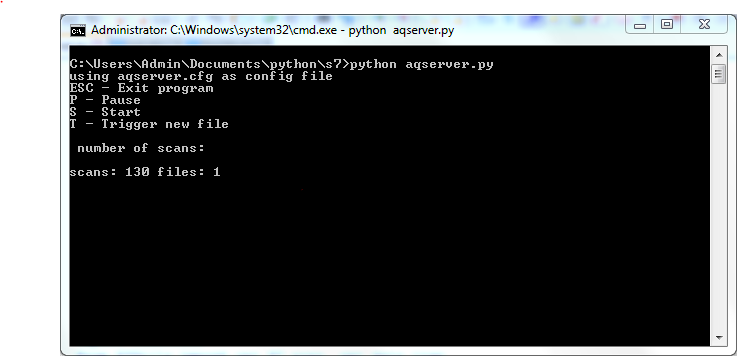
\includegraphics{usage1.png}\hfill}

As you can see in the picture above, the program is displaying some options plus the number of scans in the current data file and the number of data files recorded so far.
The options that you can use are as follows:
\begin{itemize}
\item {} 
ESC - Exit program : When you hit the ``ESC'' key the current file will be saved and then the program stops.

\item {} 
P - Pause: recording can be paused with the ``p'' key, meaning nothing will be read from the PLC and nothing will be written to the file. This can be useful if you have a break in production, but you still want the file to be continued.

\item {} 
S - Start: When program was paused or when config item autostart  is set to 0 then you can start/continue recording with  key `S''.

\item {} 
T - Trigger new file: With the ``t'' key you can manually raise a trigger. The actual data file will be stored and a new file will be started, indicated by the increasing number of files. Also number of scans start with 1 again.

\end{itemize}


\section{Using Windows installer version}
\label{usage:using-windows-installer-version}
When you have installed Aqserver using the Wondows installer, then usage is slightly different. You also might not have a working python environment installed. The installer installs the aqserver exe to  the directory ``C:\textbackslash{}Program Files (x86)\textbackslash{}Aqserver\textbackslash{}''. An example config file and a Windows / DOS batch file is copied to the ''..\textbackslash{}My Documents\textbackslash{}Aqserver\textbackslash{}'' directory. Once you have defined your config file you should edit a copy of the batch file accordingly, so that aqserver will be started using your new config file.
Contents of the batch file:

\begin{Verbatim}[commandchars=\\\{\}]
\PYGZdq{}C:\PYGZbs{}Program Files (x86)\PYGZbs{}Aqserver\PYGZbs{}aqserver.exe\PYGZdq{} \PYGZhy{}c \PYGZdq{}path\PYGZus{}to\PYGZbs{}test.cfg\PYGZdq{}
pause
\end{Verbatim}

Change path and name of your config file. Then Aqserver can be started with double clicking the batch file in Windows Explorer.


\chapter{Running multiple instances}
\label{instance:running-multiple-instances}\label{instance::doc}
If you have 2 (or more..) PLCs you want to monitor, you can do so, by running 2 separate
instances of aqserver:

Create a second config-file, containing the data required for the second connection.

\begin{notice}{note}{Note:}
Make sure you use a datafile name that is different to the other instance(s).
\end{notice}
\begin{itemize}
\item {} 
use a different name for the config-file

\item {} 
in the config-file set a different datafile name

\item {} 
start acqserver from the commandline, using the -c option

\item {} 
e.g. in Windows run:

\end{itemize}

\begin{Verbatim}[commandchars=\\\{\}]
\PYGZgt{}python aqserver.py \PYGZhy{}c my\PYGZus{}new\PYGZus{}config\PYGZus{}file.cfg
\end{Verbatim}

If you have installed Aqserver with the provided Windows installer, you can use the batch file(s) in your ''..\textbackslash{}My Documents\textbackslash{}Aqserver\textbackslash{}'' folder to start the program. (See also ``Installation'' section of this manual). For every instance create a batch file that contains the correct settings for the used config file.


\chapter{Problems}
\label{problems:problems}\label{problems::doc}
When program exits unexspected or with a message, or when program crashes, then you should turn on debugging. By default debugging is off. To run the program with debugging enabled open your config file and set
configuration value ``dbglevel'' to a value \textgreater{}0. (See below). 1 for INFO is the most verbose level. If you face problems / errors set at least to 3.

\begin{Verbatim}[commandchars=\\\{\}]
\PYG{c}{\PYGZsh{}\PYGZsh{}\PYGZsh{}\PYGZsh{}\PYGZsh{}\PYGZsh{}\PYGZsh{}\PYGZsh{}\PYGZsh{}\PYGZsh{}\PYGZsh{}\PYGZsh{}\PYGZsh{}\PYGZsh{}\PYGZsh{}\PYGZsh{}\PYGZsh{}\PYGZsh{}\PYGZsh{}\PYGZsh{}\PYGZsh{}\PYGZsh{}\PYGZsh{}\PYGZsh{}\PYGZsh{}\PYGZsh{}\PYGZsh{}\PYGZsh{}\PYGZsh{}\PYGZsh{}\PYGZsh{}\PYGZsh{}\PYGZsh{}\PYGZsh{}\PYGZsh{}\PYGZsh{}\PYGZsh{}\PYGZsh{}\PYGZsh{}\PYGZsh{}\PYGZsh{}\PYGZsh{}\PYGZsh{}\PYGZsh{}\PYGZsh{}\PYGZsh{}\PYGZsh{}\PYGZsh{}\PYGZsh{}\PYGZsh{}\PYGZsh{}\PYGZsh{}\PYGZsh{}\PYGZsh{}\PYGZsh{}\PYGZsh{}\PYGZsh{}\PYGZsh{}\PYGZsh{}\PYGZsh{}\PYGZsh{}\PYGZsh{}\PYGZsh{}\PYGZsh{}\PYGZsh{}\PYGZsh{}\PYGZsh{}\PYGZsh{}\PYGZsh{}\PYGZsh{}\PYGZsh{}\PYGZsh{}\PYGZsh{}\PYGZsh{}\PYGZsh{}\PYGZsh{}\PYGZsh{}\PYGZsh{}\PYGZsh{}}
\PYG{c}{\PYGZsh{} debug settings}
\PYG{c}{\PYGZsh{}\PYGZsh{}\PYGZsh{}\PYGZsh{}\PYGZsh{}\PYGZsh{}\PYGZsh{}\PYGZsh{}\PYGZsh{}\PYGZsh{}\PYGZsh{}\PYGZsh{}\PYGZsh{}\PYGZsh{}\PYGZsh{}\PYGZsh{}\PYGZsh{}\PYGZsh{}\PYGZsh{}\PYGZsh{}\PYGZsh{}\PYGZsh{}\PYGZsh{}\PYGZsh{}\PYGZsh{}\PYGZsh{}\PYGZsh{}\PYGZsh{}\PYGZsh{}\PYGZsh{}\PYGZsh{}\PYGZsh{}\PYGZsh{}\PYGZsh{}\PYGZsh{}\PYGZsh{}\PYGZsh{}\PYGZsh{}\PYGZsh{}\PYGZsh{}\PYGZsh{}\PYGZsh{}\PYGZsh{}\PYGZsh{}\PYGZsh{}\PYGZsh{}\PYGZsh{}\PYGZsh{}\PYGZsh{}\PYGZsh{}\PYGZsh{}\PYGZsh{}\PYGZsh{}\PYGZsh{}\PYGZsh{}\PYGZsh{}\PYGZsh{}\PYGZsh{}\PYGZsh{}\PYGZsh{}\PYGZsh{}\PYGZsh{}\PYGZsh{}\PYGZsh{}\PYGZsh{}\PYGZsh{}\PYGZsh{}\PYGZsh{}\PYGZsh{}\PYGZsh{}\PYGZsh{}\PYGZsh{}\PYGZsh{}\PYGZsh{}\PYGZsh{}\PYGZsh{}\PYGZsh{}\PYGZsh{}\PYGZsh{}}
\PYG{p}{[}\PYG{n}{debug}\PYG{p}{]}

\PYG{c}{\PYGZsh{} debug level}
\PYG{c}{\PYGZsh{} set logging level to debug, write program actions}
\PYG{c}{\PYGZsh{} to logfile}
\PYG{c}{\PYGZsh{} 0 \PYGZhy{} no logging}
\PYG{c}{\PYGZsh{} 1 \PYGZhy{} log INFO messages (default setting)}
\PYG{c}{\PYGZsh{} 2 \PYGZhy{} log WARNING messages}
\PYG{c}{\PYGZsh{} 3 \PYGZhy{} log DEBUG messages}
\PYG{c}{\PYGZsh{} 4 \PYGZhy{} log ERROR messages}
\PYG{c}{\PYGZsh{} 5 \PYGZhy{} log CRITICAL messages}
\PYG{c}{\PYGZsh{} 6 \PYGZhy{} log EXCEPTION messages}
\PYG{n}{dbglevel} \PYG{o}{=} \PYG{l+m+mi}{0}
\end{Verbatim}

Then you should start the program again and after program has ended (again) you should check the log file in the sub directory log. There you should find some more detailed information why the program won't run.
Adjust (probably) your configuration and try to run again.

Problems can be caused by:
\begin{itemize}
\item {} 
PLC cannot be reached with communication parameters provided

\item {} 
value in your list does not exist in PLC

\item {} 
typo in configuration values

\end{itemize}

If you still can't manage to make it run, send a copy of your logfile and the config file to my mail address (aqserver at taxis-instruments dot de).


\section{Frequently asked questions}
\label{problems:frequently-asked-questions}
None so far. This will be updated as questions arise. Post your questions in the contact form on my homepage or send mail to  \textless{}aqserver at taxis-instruments dot de\textgreater{}


\chapter{Introduction to Kst2}
\label{kst::doc}\label{kst:introduction-to-kst2}
Kst2 is an open source graph and plot creator and visualizer. The program can be downloaded from from \href{https://kst-plot.kde.org}{https://kst-plot.kde.org} . Most recent Windows version is 2.08.
On the homepage of the program some tutorial videos are provided. Maybe take a look at these before starting to use Aqserver and Kst2.


\section{Usage}
\label{kst:usage}
{\hfill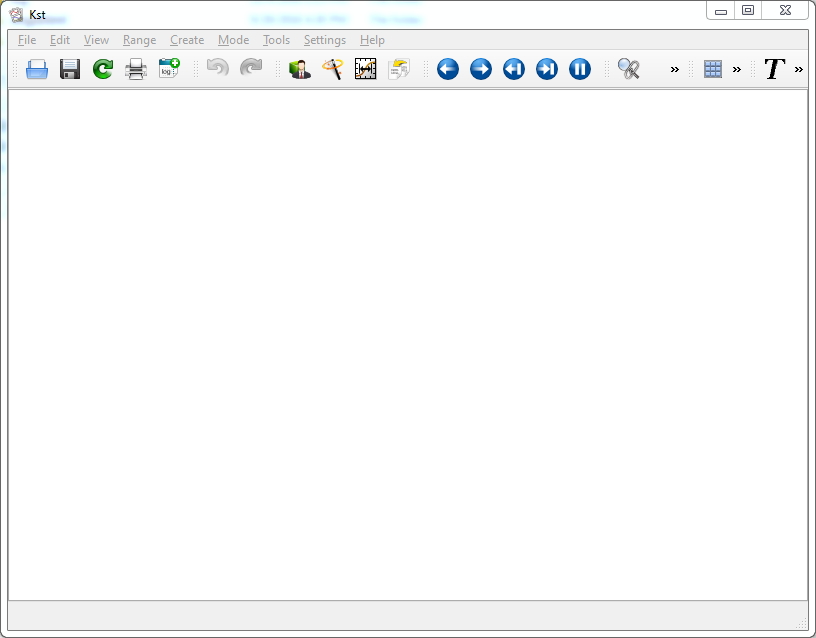
\includegraphics[width=12cm]{main.png}\hfill}

The easiest way to use Kst2 as an online chart visualizer together with Aqserver is to start with the data wizard.

\begin{notice}{note}{Note:}
You can start the data wizard several times, also with the same file, when you want to add more graphs to your display. Also if you run multiple instances of Aqserver you can pick a different datafile.
\end{notice}

Start it by clicking the following icon:

{\hfill
\includegraphics{wizard.png}\hfill}

{\hfill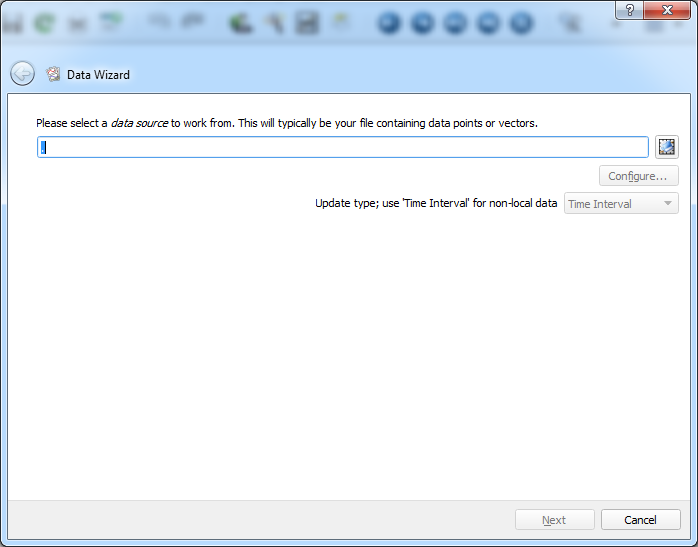
\includegraphics[width=12cm]{wiz1.png}\hfill}

The data wizard window will popup where you must select the active data file (this will be in your sub directory data ). Browse to the file to select it and then click the configure button.

{\hfill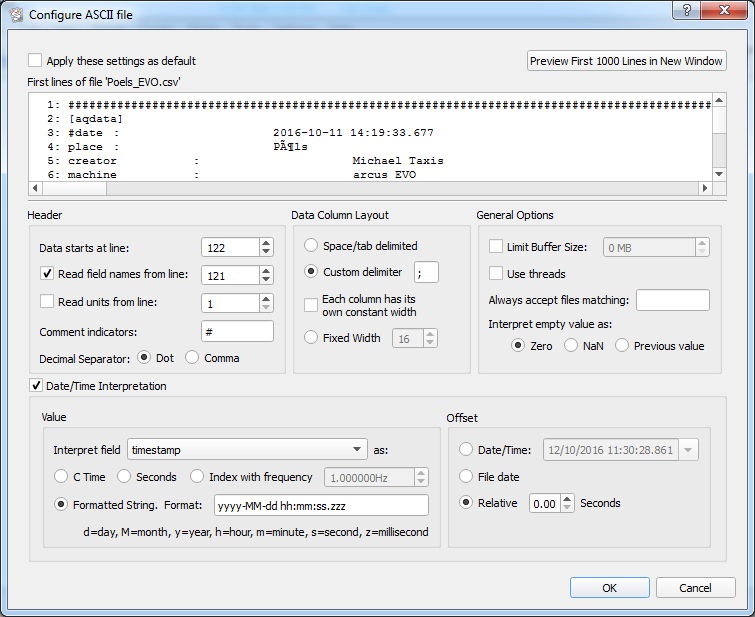
\includegraphics[width=12cm]{wiz2.png}\hfill}

The ``configure ASCII file'' window will popup. Here you must configure the properties of your data file. Values you must adjust include:
\begin{itemize}
\item {} 
Data starts at line: scroll down the window showing your datafile until you reach the first recorded values. Note the number and put into the required field. If the first data line is not shown, try the button ``Preview first 1000 lines in new window''.

\item {} 
Obviously the ``Read field names from:'' option must activated and the acording line number must be entered (see above value - 1)

\item {} 
set the decimal separator

\item {} 
set the Custom delimiter to the one you have used in the datafile

\item {} 
activate ``Date/Time Interpretation''

\item {} 
scroll down the ``Interpret field as'' and pick the value timestamp. (If no selection is shown, exit with ``Ok'' and enter configuration again, then try to pick timestamp).

\item {} 
activate ``formatted string'' and set the format to ``yyyy-MM-dd hh:mm:ss.zzz''. Then our timestamp will be interpreted correctly.

\end{itemize}

Leave the window with ok. Set the update type to either time interval or you can try change detection. When using an already recorded archive you can use no update. Then click ``Next'' in the Data Wizard window.

{\hfill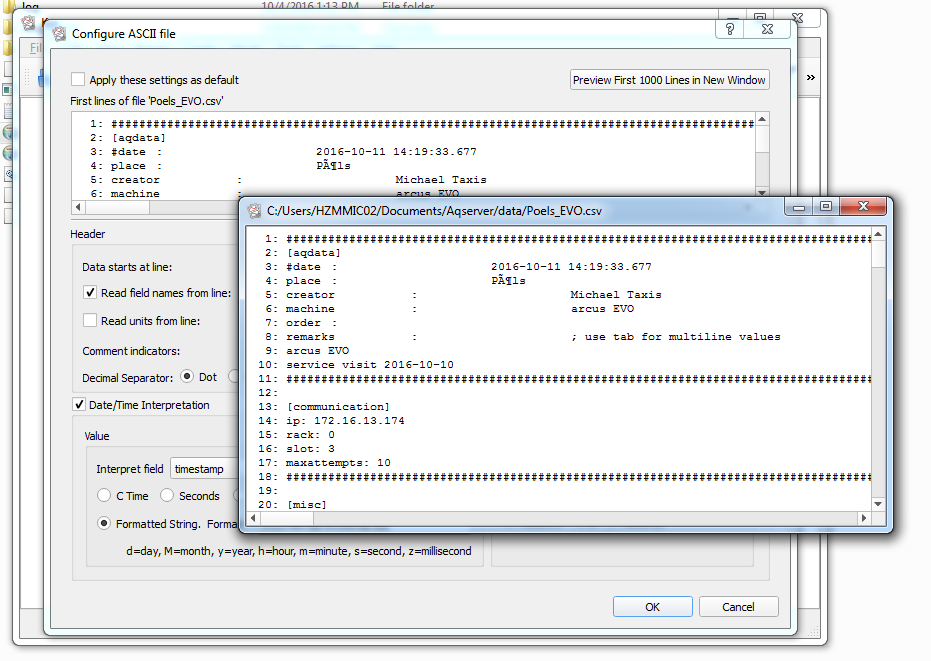
\includegraphics[width=12cm]{wiz3.png}\hfill}

Data wizard with  ``Preview first 1000 lines in new window''.

{\hfill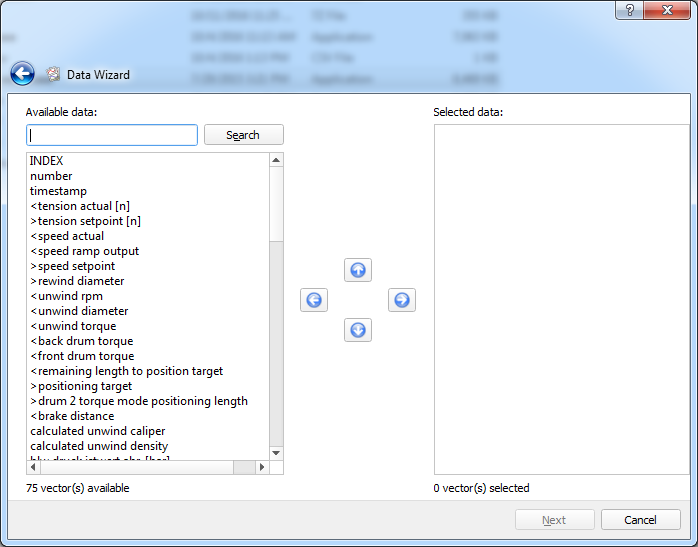
\includegraphics[width=12cm]{wiz4.png}\hfill}

Pick the values you want to be shown in a graph and move them to the right window with the arow buttons. Click next

{\hfill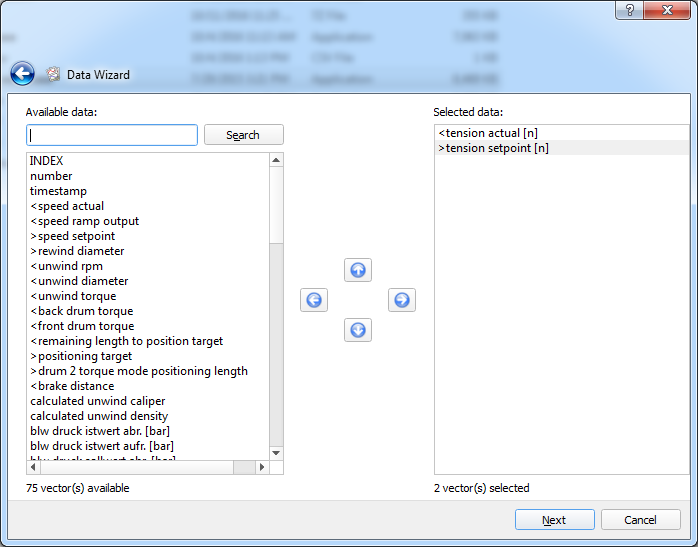
\includegraphics[width=12cm]{wiz5.png}\hfill}

Same with some values selected.

{\hfill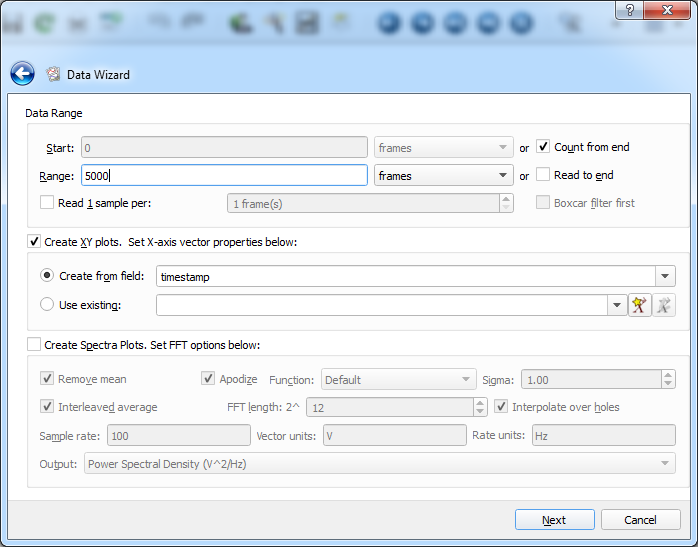
\includegraphics[width=12cm]{wiz6.png}\hfill}

Experiment a little bit with data range settings. Activate ``Create XY-plots''. For X-axis vector we select our field ``timestamp''. Click next.

{\hfill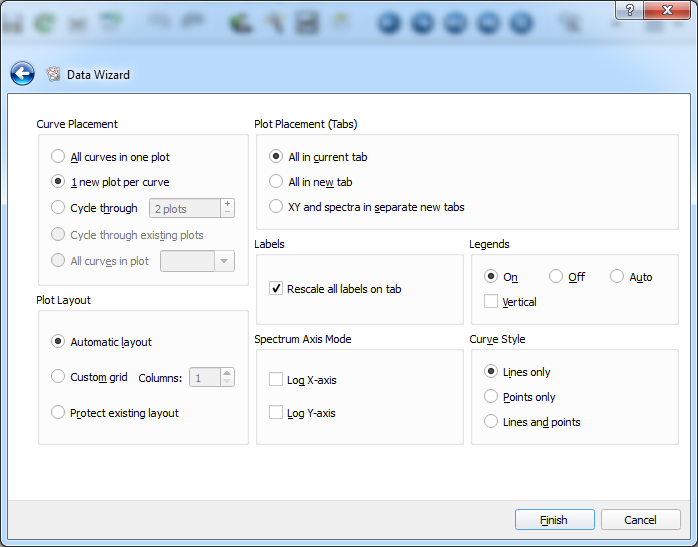
\includegraphics[width=12cm]{wiz7.png}\hfill}

Then we setup the appearance of the graphs, either in one plot or 1 plot per curve.

{\hfill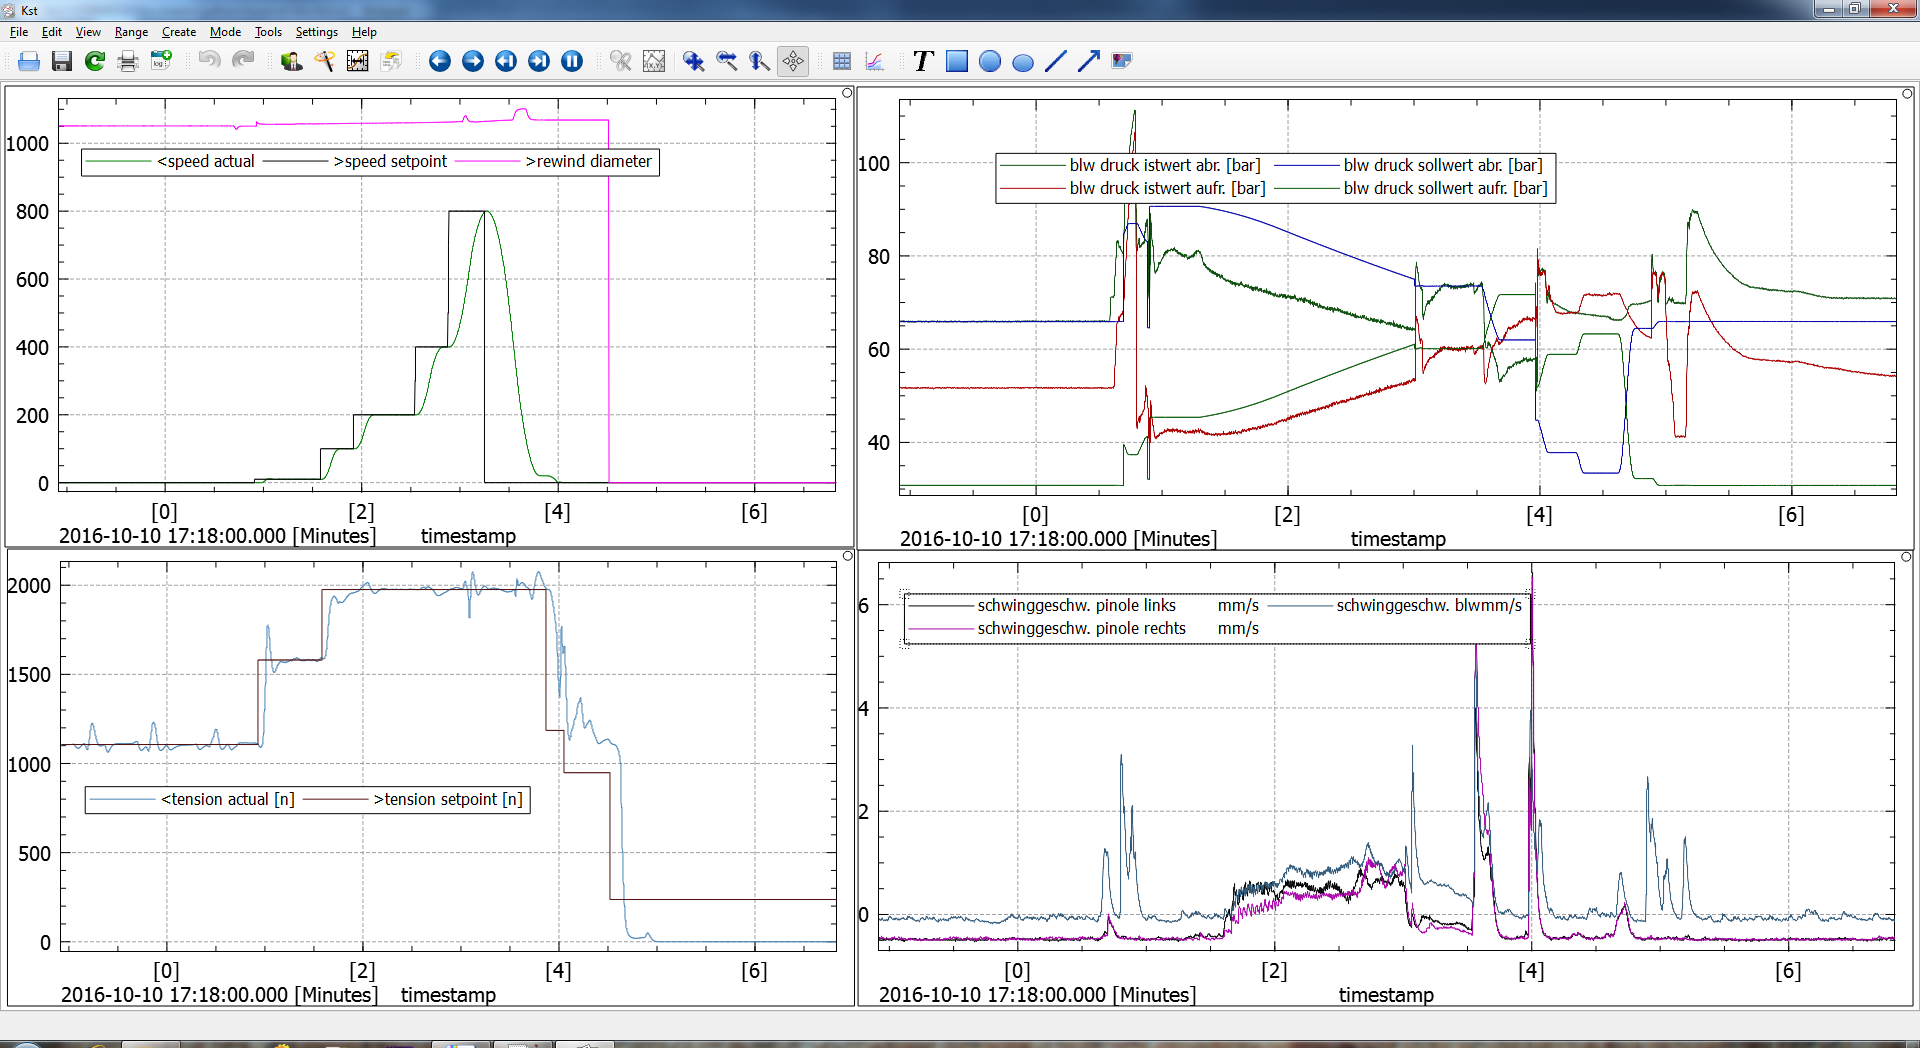
\includegraphics[width=15cm]{offline.png}\hfill}

Finally we will be shown our recorded values. If you have picked an updating file, the curves will also update.

\begin{notice}{note}{Note:}
When a trigger has been raised that starts a new datafile use the green round arrow key to reload your datafile. Otherwise Kst2 will not update with the new file.
\end{notice}

For further information about Kst2 try their documentation, forums etc.


\chapter{Changelog}
\label{changelog::doc}\label{changelog:changelog}
13 October 2016
\begin{itemize}
\item {} 
updated docs

\item {} 
created new installer using pyinstaller and NSIS. Problems before with py2exe.

\end{itemize}

11 October 2016
\begin{itemize}
\item {} 
added check for maximum records (from config) to avoid files getting too big

\item {} 
added try ..except for reading config file

\end{itemize}

06 October 2016
\begin{itemize}
\item {} 
PrgUtils.py: added get username for all OS (Windows, Linux, MacOS)

\item {} 
aqserver.py: change data and log directory, depending on OS. In Windows this will be sub directories of .. My Documents\textbackslash{}Aqserver folder, in Linux/MacOS this will be in current users home directory (//home//user//Aqserver//..)

\end{itemize}

05 October 2016
\begin{itemize}
\item {} 
NSIS: tried to make setup.exe for Windows

\item {} 
aqserver.py: added manual trigger always possible

\item {} 
aqserver.py: added check for variables, and exit with config fault, problem to logfile

\end{itemize}

30 September 2016
\begin{itemize}
\item {} 
updating docs

\item {} 
aqserver.py: check if argument for config file is list or string

\item {} 
aqserver.py: added purging log directory, when debug is 0 (= no debugging), only actual logfile remains, with entry program start and end

\item {} 
aqserver.py: improved error detection, connect and disconnect of client

\end{itemize}

29 September 2016
\begin{itemize}
\item {} 
updated docs

\item {} 
compiled to exe with py2exe

\item {} 
can test now with local Snap7 server

\item {} 
added verification for configfile, data dir and log dir, if a dir is missing it will be created

\item {} 
fixed keypress problem, program was not responding to every keypress

\end{itemize}

15 September 2016
\begin{itemize}
\item {} 
added try..except for communication error, program exits normal now, with message to user and logfile

\item {} 
when client was already connected program tries to disconnect and to connect again (no exit)

\item {} 
when scantime is set to 0 then program scans as fast as possible (no sleep)

\end{itemize}

28 November 2015
\begin{itemize}
\item {} 
modified aqserver(none OOP version), can now use directory structure yearmonthday  for saved files

\end{itemize}

11 August 2015
\begin{itemize}
\item {} 
started refactoring and making OOP aware, with acqserver class (not yet finished)

\end{itemize}

10 August 2015
\begin{itemize}
\item {} 
tested and corrected trigger functionality

\item {} 
tested S7 300 with plcsim and nettoplcsim

\end{itemize}

07 August 2015
\begin{itemize}
\item {} 
added filecopy routines to PrgUtils

\item {} 
added trigger functionality to server (aqserver.py)

\end{itemize}

06 August 2015
\begin{itemize}
\item {} 
added config section for debug, with settings for debug level, logfile

\item {} 
corrected error in endless loop that creates string with values

\item {} 
create header template at start, that can be copied to further data files in case of trigger

\item {} 
removed all sys.args, only*c configfile remains, all other settings in config file

\item {} 
tried to start 2 instances of program

\end{itemize}
\begin{itemize}
\item {} 
use different configfile

\item {} 
set different recording filename

\item {} 
when started from 2 cmd environments with*c parameter and different configfile, it works!

\end{itemize}
\begin{itemize}
\item {} 
tested filecopy, rename, append, replace in file as preparation for trigger event actions

\end{itemize}

05 August 2015
\begin{itemize}
\item {} 
added data file name to config, so we can start aqserver several times using different settings, when scanning several PLCs

\end{itemize}


\chapter{Licensing}
\label{license::doc}\label{license:licensing}
Aqserver is distributed as python source code or Windows setup program under Lesser General Public License version 3.0 (LGPLv3)

Basically this means that you can distribute your commercial software linked with Aqserver without the requirement to distribute the source code of your application and without the requirement that your application be itself distributed under LGPL.

A small mention to the project or the author is however appreciated if you include it in your applications.


\section{Disclaimer of Warranty}
\label{license:disclaimer-of-warranty}
THERE IS NO WARRANTY FOR THE PROGRAM, TO THE EXTENT PERMITTED BY APPLICABLE LAW. EXCEPT WHEN OTHERWISE STATED IN WRITING THE COPYRIGHT HOLDERS AND/OR OTHER PARTIES PROVIDE THE PROGRAM ``AS IS'' WITHOUT WARRANTY OF ANY KIND, EITHER EXPRESSED OR IMPLIED, INCLUDING, BUT NOT LIMITED TO, THE IMPLIED WARRANTIES OF MERCHANTABILITY AND FITNESS FOR A PARTICULAR PURPOSE. THE ENTIRE RISK AS TO THE QUALITY AND PERFORMANCE OF THE PROGRAM IS WITH YOU. SHOULD THE PROGRAM PROVE DEFECTIVE, YOU ASSUME THE COST OF ALL NECESSARY SERVICING, REPAIR OR CORRECTION.

IF ANYONE BELIEVES THAT, WITH THIS WEBSITE OR WITH AQSERVER PROJECT SOME COPYRIGHTS HAVE BEEN VIOLATED, PLEASE EMAIL US, AND ALL THE NECESSARY CHANGES WILL BE MADE.



\renewcommand{\indexname}{Index}
\printindex
\end{document}
